\documentclass{beamer}
% \documentclass[handout]{beamer}
\usetheme{focus}
\usepackage{graphicx}

\title{Anonymous Walk Embedding}
\subtitle{ICML'18, Sergey Ivanov \& Evgeny Burnaev}
\author{Hoang NT}
\titlegraphic{
\includegraphics[scale=0.3]{imgs/anon.png}}
\institute{Murata Laboratory \\ Tokyo Tech \vspace{4em}}
\date{2019/01/10}

\begin{document}
    \begin{frame}
        \maketitle
    \end{frame}

    \begin{frame}{Overview}
        \tableofcontents
    \end{frame}

    \section{Graphs Distance}

    \subsection{Comparing Graphs}

    \begin{frame}{Why do we need graph distance?}
        Given a network modeled as a graph, there are many questions to ask. For example:
        \pause
        \begin{itemize}
            \item Is the graph connected? 
            \item How to maximize vertices independent set?
            \item Where is the best graph cut?
            \item How to describle the graph mathematically?
            \item How to do all above if the graph is "large"?
        \end{itemize}
        \pause
        \vspace{1em}
        \begin{block}{How to answer (some of) the questions above?}
            Defining a scalable graph distance is a key challenge that would 
            give us an advantage in analysis.
        \end{block}
    \end{frame}

    \begin{frame}{Example problems}
        \begin{columns}
            \column{0.49\textwidth}
                \begin{exampleblock}{Graph classification}
                    Using measure distance between graphs, we can have better 
                    machinery to understand new graph designs.
                \end{exampleblock}

                \pause

                \begin{exampleblock}{Graph modeling}
                    Combining random graph modelings
                    with generative neural networks,
                    we can generate new designs for materials, drugs, 
                    and complex systems.
                \end{exampleblock}

            \column{0.49\textwidth}
                Molecules and nano-structures are often modeled as graphs:
                \begin{figure}
                    \centering
                    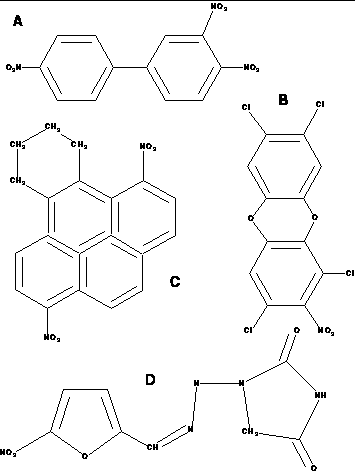
\includegraphics[width=0.7\textwidth]{imgs/mutagens.png}
                    \caption{How do we compare these molecules?}
                    \label{fig:mutag_9_11}
                \end{figure}
        \end{columns}
    \end{frame}

    \begin{frame}{Types of graph distance}
        There are many definitions for graph distances depending on the specific
        problem.
        \pause
        \begin{enumerate}
            \item Exact topological distances:
            \pause
            \begin{itemize}
                \item Edit distance (Hamming distance)
                \pause
                \item Homomophism count for some smaller graph $\mathcal{F}$
                \pause
                \item Frieze-Kannan cut-norm
                \pause
                \item etc.
            \end{itemize}
            \item Other (approximate) distances:
            \pause
            \begin{itemize}
                \item Spectral gap and graph spectrum
                \pause
                \item Graph features-based distance (L1,2 of features)
                \pause
                \item etc.
            \end{itemize}
        \end{enumerate}
    \end{frame}

    \subsection{Main Objective of the Paper}

    \begin{frame}{This paper}
        In this paper: "Anonymous Walk Embedding", the authors addressed the 
        \textcolor{example}{graph distance} design by an modified version
        of approximate homomomophism counting.

        \vspace{1em}

        \pause

        \begin{block}{Main experiment}
            \textbf{Input}: A set of graphs, each associated with a label. \\
            \textbf{Output}: A set of (task-agnostic) vector representations
            for each graph in the dataset. These representations later used as
            feature vectors for the graph classification task.
        \end{block}
    \end{frame}

    \section{Embedding Methods}

    \subsection{Anonymous Walk}

    \begin{frame}{Anonymous Walk definition}
       \begin{block}{Definition 1: Anonymous Walk}
            \textcolor{example}{An Anonymous Walk} is a random walk where 
            vectices are replaced by their 
            \emph{appearance orders in the walk}. \\
            \textbf{(Def. 2 in the paper)} If $\omega = (v_1, v_2, ... , v_k)$ is a
            random walk, then its corresponding Anonymous Walk is a sequence
            of integers $a = (f(v_1), f(v_2), ... , f(v_k))$ where the integer 
            $f(v_i) = \min pos(v_i, w)$.
       \end{block} 

        \begin{figure}
            \centering
            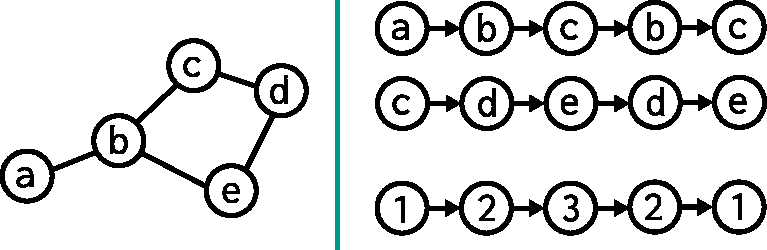
\includegraphics[height=6em]{imgs/anonwalkexample.pdf}
            \caption{Anonymous Walk Example.}
            \label{fig:anonwalkexample}
        \end{figure}
    \end{frame}

    \begin{frame}{Assumtions and intuition}
        This paper was built on the results (Theorem 1 and 1') of 
        \cite{micali2016reconstructing}:

        \begin{block}{Theorem 1 (Micali et al., 2016)}
            Let $n$ be a number of vectices in $B(v,r)$ and $m$ is the number
            of edges. One can reconstruct $B(v,r)$ in time $O(n^2)$ with 
            $O(n^2)$ oracale access to $(\mathcal{D}_1, ... , \mathcal{D}_l)$,
            where $l = O(m)$. Moreover, the reconstruction algorithm only makes 
            membership queries to $\text{supp}(\mathcal{D}_i)$ for $i \in [l]$.
        \end{block}

        \vspace{1em}

        The author of AWE assumes that if one could reconstruct the topological
        ball $B(v,r)$ around vertex $v$ by the distribution of Anonymous Walks, 
        one could approximately say the samething about the whole graph. (?)
    \end{frame}

    \subsection{Graph Features}

    \begin{frame}{Method 1: Features Based}
       \begin{block}{Definition 2: AW-FB}
            \textbf{(Def. 3 in the paper)} Feature Based Anonymous Walk:
            Let $\mathcal{A}_l = (a_1, a_2, ..., a_\eta)$ be the set of all
            possible anonymous walk of length $l$. \emph{Anonymous Walk 
            Embedding} of a graph $G$ is the vector $f_G$ of size $\eta$, 
            whose $i$-th component corresponds to a probability $p(a_i)$, 
            of having anonymous walk $a_i$ in the graph $G$:
            $$ f_G = (p(a_1), p(a_2), ..., p(a_\eta)) $$
       \end{block} 

       The probability $p(a_i)$ is empirically estimated using random sampling. 
       The confident intervals for $m$ samples is given by a similar work using
       graphlet kernel for graph comparisons \cite{shervashidze2009efficient}.
    \end{frame}

    \begin{frame}{Method 2: Data Driven}
       \begin{block}{Definition 3: AW-DD}
            Data Driven Anonymous Walk: Let an Anonymous Walk starting from 
            a vertex $u$ be analogous to a "word" and the whole graph be 
            analoguous to a "document". The authros now use document embedding 
            in the NLP setting to obtain the graph vector by maximizing the
            average log-probability:
            $$ \frac{1}{T} \sum_{t=\Delta}^{T-\Delta} \log p(w_t | \Delta(w_t), d) $$
       \end{block} 

       \vspace{1em}

       In here, a neighboorhood $\Delta{w_t}$ is the set of Anonymous Walks
       rooted at the same vertex.
    \end{frame}

    \begin{frame}{Method 2: Data Driven}
        \begin{columns}
            \column{0.49\textwidth}
                \begin{figure}
                    \centering
                    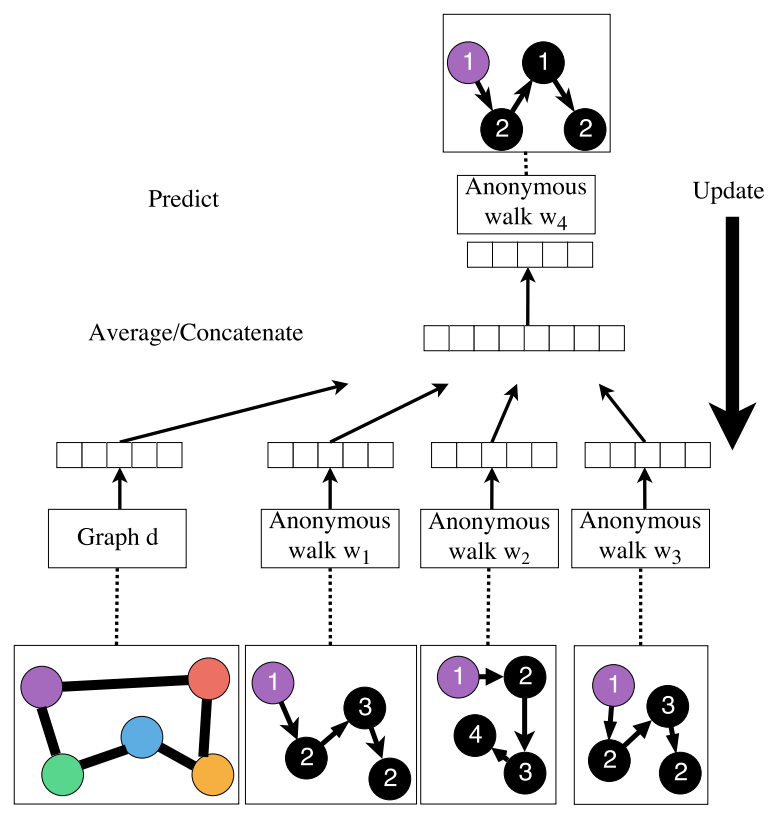
\includegraphics[width=\textwidth]{imgs/framework.png}
                    \caption{Data Driven Framework. \cite{pmlr-v80-ivanov18a}}
                    \label{fig:awdd}
                \end{figure}

            \column{0.49\textwidth}
                \pause
                \begin{exampleblock}{Step 1: Create data}
                    Starting at each vertex, 
                    perform $T$ anonymous walks of length $l$. 
                \end{exampleblock}
                \pause
                \begin{exampleblock}{Step 2: Doc2Vec}
                    Training a doc2vec model with anonymous walks as words and
                    the graph as the document. Local context is the set $T$
                    walks of each vertex.
                \end{exampleblock}
        \end{columns}
    \end{frame}

    \section{Experiments \& Results}

    \subsection{Datasets \& State-of-the-art}

    \begin{frame}{Datasets}
        \begin{table}
            \centering
            \begin{tabular}{llllll}
                \textbf{Datasets} & \textbf{Source} & \textbf{\#Graphs} &
                \textbf{Classes (max)} & \textbf{N/E Avg.}\\\hline
                COLLAB & Social & 5000 & 3 (2600) & 74.49 / 4914.99\\
                IMDB-B & Social & 1000 & 2 (500) & 19.77 / 193.06\\
                IMDB-M & Social & 1500 & 3 (500) & 13 / 131.87\\
                RE-B & Social & 2000 & 2 (1000) & 429.61 / 995.50\\
                RE-M5K & Social & 4999 & 5 (1000) & 508.5 / 1189.74\\
                RE-M12K & Social & 12000 & 11 (2592) & 391.4 / 913.78\\
                Enzymes & Bio & 600 & 6 (100) & 32.6 / 124.3\\
                DD & Bio & 1178 & 2 (691) & 284.31 / 715.65\\
                Mutag & Bio & 188 & 2 (125) & 17.93 / 19.79\\
            \end{tabular}
            \caption{Datasets used in the paper.}
            \label{tab:datasets}
        \end{table}
        \vspace{-0.5em}
        10-fold cross validation is used for each dataset and each 
        parameter setting of their methods. 
    \end{frame}

    \begin{frame}{Competitors}
        There are two groups of other methods:
        \pause
        \begin{enumerate}
            \item Data Driven:
            \begin{itemize}
                \pause
                \item \textbf{PSCN}: Patchy-San (Niepert et al., 2016) - 
                Trains a convolutional neural network from generated graph
                neighboorhood.
                \pause
                \item \textbf{DGK}: Deep Graph Kernel (Yanardag et al., 2015) - 
                Learn a positive semidefinite matrix to weight the relationship
                between substructures.
            \end{itemize}
            \pause
            \item Features Based:
            \begin{itemize}
                \pause
                \item \textbf{WL}: Weisfeiler-Lehman Kernel (Shervashidze
                et al., 2011) - Construct graph features from the subtree 
                patterns of a graph.
                \pause
                \item \textbf{GK}: Graphlet Kernel (Shervashidze et al., 2009)
                - Construct graph features from graphlets (\~motifs).
                \pause
                \item \textbf{ER}: Exponential Random Walk Kernel 
                (Gartner et al., 2003).
                \item \textbf{kR}: k-step Random Walk Kernel 
                (Sugiyama et al., 2015).
            \end{itemize}
        \end{enumerate}
    \end{frame}

    \subsection{Results}

    \begin{frame}{Results: Social Networks}
        \begin{figure}
            \centering
            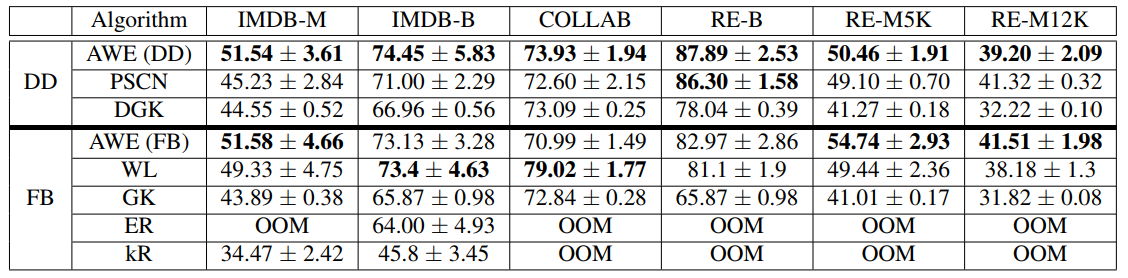
\includegraphics[width=\textwidth]{imgs/result_social.png}
            \caption{Classification accuracy for social networks
            (Table 2 \cite{pmlr-v80-ivanov18a})}
            \label{fig:socialresults}
        \end{figure}
    \end{frame}

    \begin{frame}{Results: Bio Datasets}
        \begin{figure}
            \centering
            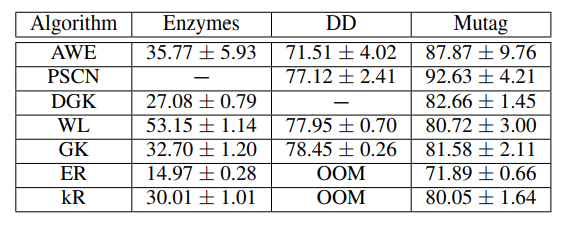
\includegraphics[width=0.65\textwidth]{imgs/result_bio.png}
            \caption{Classification accuracy for Bio datasets
            (Table 4 \cite{pmlr-v80-ivanov18a})}
            \label{fig:bioresults}
        \end{figure}
    \end{frame}

    \subsection{Conclusion}

    \begin{frame}{Conclusion}
        \pause
        The authors used \textbf{anonymous walks} to create embedding 
        vector to a given graph. There are two ways to create such vector:
        \pause
        \begin{enumerate}
            \item Count the number of unique anonymous walks.
            \pause
            \item Use \texttt{doc2vec} algorithm to learn the embedding vector.
        \end{enumerate}
        \pause
        Advantage:
        \pause
        \begin{itemize}
            \item Scalable whole graph embedding algorithm.
            \pause
            \item Open to many different ML tasks.
            \pause
            \item The algorithm is highly customizable to learn node and 
            subgraph representations.
        \end{itemize}
        \pause
        Disadvantage:
        \pause
        \begin{itemize}
            \item Doc2Vec algorithm takes very long time to run 
            (2.7hrs for 100 epochs of Mutag on my machine).
            \pause
            \item Theorem 1 is trivial. There is no guarantee for the
            assumption that similar graphs exhibit similar distribution of
            anonymous walk.
        \end{itemize}
    \end{frame}

    \begin{frame}[focus]
        Thanks for listening!
    \end{frame}

    \appendix
    \begin{frame}{References}
        \nocite{*}
        \bibliography{main}
        \bibliographystyle{plain}
    \end{frame}
\end{document}
